
The first step in the signal processing was to isolate the information bearing signal. The most straightforward step was hence to remove the 4MHz signal and its harmonics that arise from the main processor. The 30.8 GHz signal we are interested in is preserved as shown in Figure \ref{figure:harmonics_removal}.

    \begin{figure*}
      \centering
      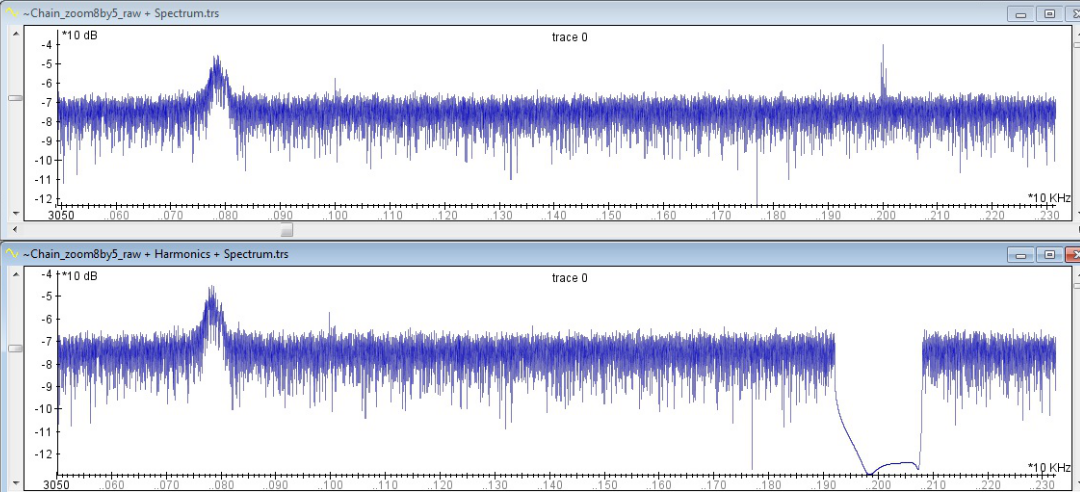
\includegraphics[scale=0.3]{img/harmonics_removal.png}
      \caption{\label{figure:harmonics_removal}Removal of 4GHz harmonics.}
    \end{figure*}  

The EM signal was sampled at a very high frequency (250 Mhz to 1 GHz), and fluctuates frequently between positive and negative values. To better analyse the signal, we try to obtain the absolute value of the signal envelope by using the ``Sync Resample" module which  resamples the original signal at a 30.8 MHz sample rate. Thereafter, we perform low pass filtering. 

These three steps were sufficient to produce a sufficiently clear signal for simple side channel analysis. In the Lim-Lee algorithm, a single scalar multiplication has many rounds. At the beginning of each round, we observe a distinct pattern of 5 or 7 bumps as shown in Figure \ref{figure:pattern}. Here, 5 bumps indicate a 0-bit and 7 bumps indicates a 1-bit value of the nonces used in Lim-Lee. Sufficient nonce values can be obtained across approximately 50 traces (using different input points) to recreate the secret ECC scalar.

Although these three signal processing steps were sufficient, we could additionally have averaged multiple EM traces (using the same  input Point) to produce an even clearer signal, for each of the required 50 traces.

    \begin{figure*}
      \centering
      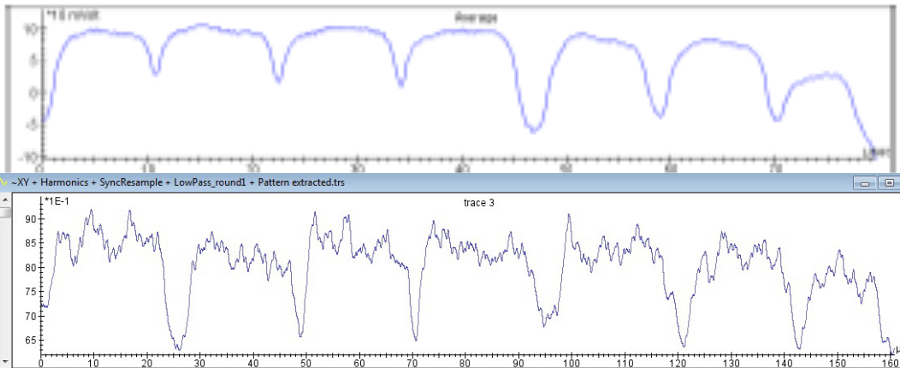
\includegraphics[scale=0.3]{img/pattern.png}
      \caption{\label{figure:pattern}The upper image was obtained from an unfiltered power trace. The lower image was our actual EM measurements after signal processing.}
    \end{figure*}  


